\subsubsection{Purpose}
The user of the application who has correctly logged in the web application or the mobile one, can view and organize the appointments into his own calendar. The system provides the user the possibility to see, create, modify or delete any appointments that he/she has inserted. In particular, the main features are as follows:
\begin{itemize}
\item View appointments: the user is given the possibility to view all the appointments, both with the general overview in the form of a grid, and the list view with appointments and the public means interleaved.
\item Create appointment: the user has to click on the specific date where he wants to add the new appointments and inserts the information below:
        \begin{enumerate}
        \item Name of appointment;
        \item Start time;
        \item End time;
        \item Recurrence (optional);
        \item Means of transport.
        \end{enumerate}
\item Modify appointment: the user simply clicks on the appointments that he has created so that he is able to update the information.
\item Delete appointment: the user through the same gesture of \textit{Modify appointment} can easily delete the appointment by clicking on the specific button.
\end{itemize}

\subsubsection{Scenario 1}
Alice, a young business consultant, plans all her appointments through the Travlendar+ application. Every Wednesday, the company decides to organize a refresher course. For this reason, she needs to add this appointment to her calendar.
Alice through the calendar interface, clicks on the first day course and adds the necessary information to create the appointment by using the form: event name, start time, end time, recurrence, means of transport. The system checks that the new appointment meets each requirement and asks Alice to confirm. Once confirmed, the event is displayed in her list of appointments. Unfortunately, the company after a few days, deletes the refresher course, so Alice wants to delete the appointment from her calendar. Alice easily accesses the event and modifies it. By clicking the corresponding button, she deletes the event and all the saved recurrences. The system asks Alice if she is really sure to perform the operation, she confirms and the event is deleted from the calendar.

\subsubsection{Scenario 2}
Bob, after correctly signing up to Travlendar+, decides to check the appointments of the day through the calendar. While he’s scrolling the appointment list, he notices that one of the places of meeting was entered incorrectly. By simply clicking on the event, Bob is able to update the information. The system checks that the updated appointment meets each requirement. After calculating the time needed to reach the place of the appointment, the system warns Bob that the travel time between the previous and the updated event is not enough to reach the place of the appointment. However, the system asks Bob if he wants to confirm or update the event. He doesn’t choose to update the event, so changes are not made. Bob accesses the event and modifies it again, but in this case, he deletes the event by clicking on the specific button. The system requires confirmation and the event is deleted form the calendar.

\subsubsection{Use case}
The use case for creating an appointment is shown in Table \ref{usecase_app}.

\begin{table}
\centering
	\begin{tabular}{|c||p{0.6\textwidth}|}
		\hline
		Name & Create appointment \\ \hline
		Actors & User \\ \hline
		Assumption & The user needs to insert a new appointment in his/her personal calendar \\ \hline
		Pre-Conditions & \begin{itemize}
			\item The user has successfully signed to the system.
			\item The user has already opened the window with the insertion form.
		\end{itemize} \\ \hline
		Flow of events & \begin{enumerate}
			\item The user creates a new appointment by inserting all the information needed in order to adding a new event correctly in his own calendar.
			\item The system checks if the appointment inserted can be successfully validated. This means that simple checks against the time (the start one should be less than the end one) and the date (should not be an expired date) are done. \textit{Note:} overlapping events check is done at a second stage. 
			\item The user is informed by a warning message about the actual validation of the appointment.
			\item The user have to confirm o reject the insertion of the appointment.
		\end{enumerate} \\ \hline
		Post-Conditions & The appointment of the user has been stored into the system in the event that he has confirmed the inclusion. \\ \hline
		Exception & An internal system error makes impossible to store the reservation data. The user is notified of the error \\ \hline		
	\end{tabular}
\caption{Use case for create appointment.}
\label{usecase_app}
\end{table}
    
\subsubsection{Sequence diagram}
The sequence diagram for creating an appointment is illustrated in Figure \ref{fig:SequenceLogin}.
\begin{figure}
	\centering
	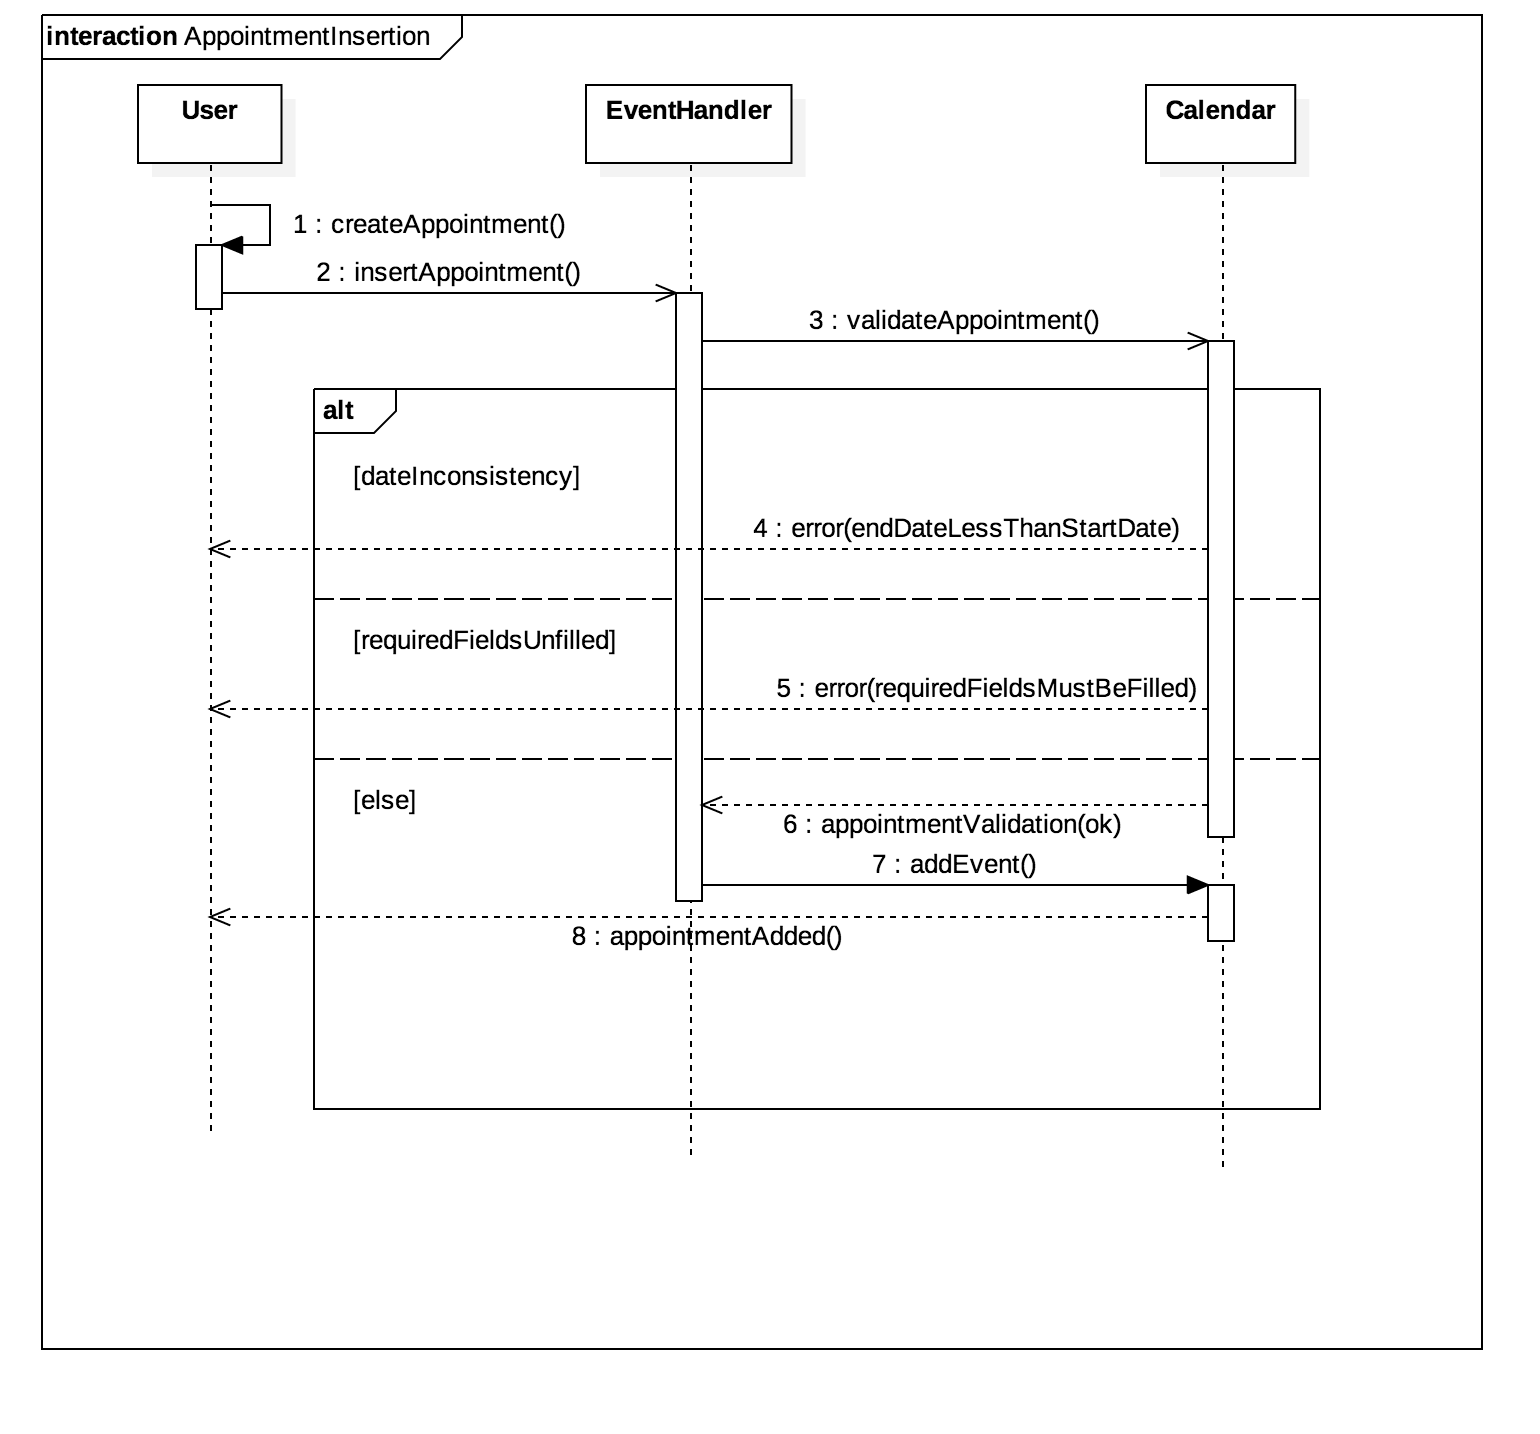
\includegraphics[width=6in]{./diagrams/AppointmentInsertion.png}
	\caption{Sequence Diagram: Create Appointment}
	\label{fig:SequenceAddApp}
\end{figure}

\subsubsection{Mockup}
The mockup of the appointments overview and the list view are shown in Figure \ref{fig:MockupAppointments} and in Figure \ref{fig:MockupListing}, the menu of the application is shown in Figure \ref{fig:MockupMenuView} and the creation of appointments is shown in Figure \ref{fig:AppointmentCreationMockup}.
\begin{figure}
	\centering
	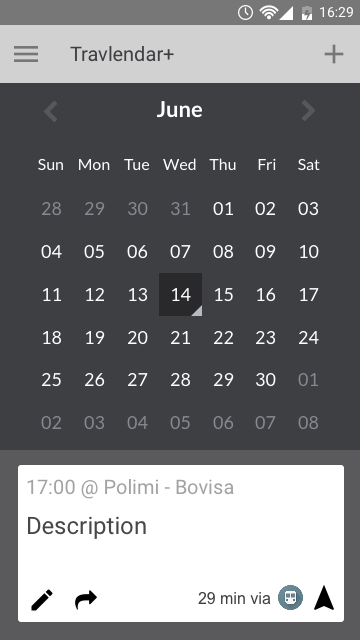
\includegraphics[width=4.5in]{./images/home.png}
	\caption{Overview appointments mockup.}
	\label{fig:MockupAppointments}
\end{figure}
\begin{figure}
	\centering
	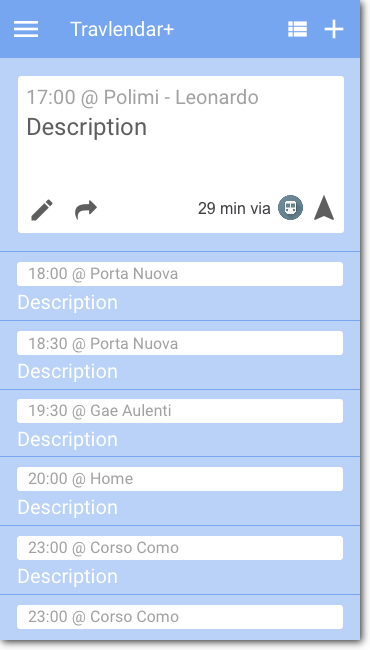
\includegraphics[width=4.5in]{./images/listing.png}
	\caption{Listing view appointments mockup.}
	\label{fig:MockupListing}
\end{figure}
\begin{figure}
	\centering
	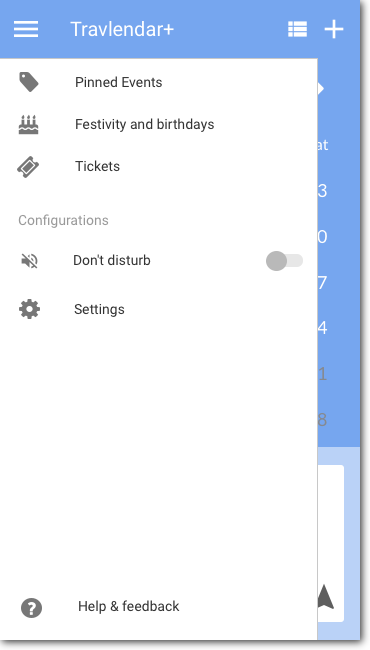
\includegraphics[width=4.5in]{./images/menu.png}
	\caption{Menu view mockup.}
	\label{fig:MockupMenuView}
\end{figure}
\begin{figure}
	\centering
	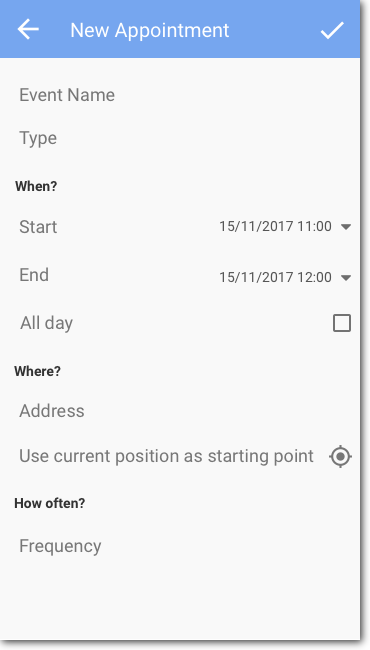
\includegraphics[width=4.5in]{./images/appointment.png}
	\caption{Creation appointment mockup.}
	\label{fig:AppointmentCreationMockup}
\end{figure}